\section{Study 2: User Behavior on the TypeBoard}

In this study, we obtained users' typing data on the TypeBoard, a touchscreen keyboard with unintentional touch rejection. Participants used the TypeBoard developed in study one. The motivation was to investigate users' typing behavior, based on which we can further improve the identification of unintentional touch.

%we recruited 16 participants and divided them into four groups equally. The first group of participants typed on the existing TypeBoard. After each group finished the experiment, we used the data to improve the TypeBoard. The following participants typed on the improved TypeBoard. That is, we explored the user behavior and improve the method through an iterative process.

\subsection{Participants}

We recruited 16 participants from the local campus (aged from xx to xx, M = xx.xx, SD = xx.xx, xx females). All the participants were righted handed and did not took part in the first study. They have used software keyboards on smartphones for not less than xx years. xx of the 20 participants were familiar with software keyboards on tablets.

%We divide the participants into five groups. Each group had four people. The five groups were well-matched in age. As a previous work did \cite{2020-QwertyRing},  we ran a program to divide the participants randomly for 1000 times and picked the five groups of which the average ages were the closest (M = xx.x, xx.x, xx.x, xx.x, xx.x, SD = xx.x, xx.x, xx.x, xx.x, xx.x). The first group of participants typed on the naive TypeBoard, while the following groups used continually improved keyboards.

%我们从本地的校园中邀请了20名用户参与实验,他们的年龄从xx岁到xx岁不等,平均数是xx,标准差是xx,其中有xx名女性。所有的用户都是右撇子,所有用户有超过xx年的手机文本输入经历,xx名用户常用平板电脑进行文本输入。这些用户没有参与过实验一。如上面所说,我们将用户分成了五组,为了保证五组用户的平衡性,我们通过程序随机模拟了10000次分组,最终确定了平均年龄最相近的分组方式,这五组的年龄平均数分别为xx,xx,xx,xx,xx,每组分别有xx,xx,xx,xx,xx名女性。

\subsection{Design and Procedure}

As figure xx shows, the experimental devices were the same as those in study one, including a Windows surface tablet and a Morph Sensel force-sensitive touchpad. The working frequency was 50 FPS. There were four sessions of text entry tasks, which also reminded the same as study one. The differences in study two are as follows. First, participants could actually enter words by typing on the touchpad. Second, the system supported unintentional touch rejection. Intentional touches would trigger keystrokes and audio feedback, while unintentional touches were ignored.
%正式实验分为四个session,分别收集了用户在填写个人信息、描述个人爱好、模拟开卷考试和看图写话这四个任务下的打字数据,我们通过拉丁方来平衡每个用户做这四个任务的顺序。如图xx所示展示了实验二的实验设置,桌面上的实验设备包含morph-sensel压力触摸板、鼠标、显示器和耳机。在本实验中,用户同样通过填写word文档的方法来完成四个文本输入任务(图xx)。和实验一不一样的是,用户在本实验中真的能够通过TypeBoard来键入字母,且打字的过程中能够听到“啪啪”的声音反馈。

【图:实验二的设置图,突出实验二中】

Before the experiment, participants warmed up by a ten-minute daily writing. Because no participant had experience with typing on a keyboard with unintentional touch rejection, we reminded the participants that they could rest their fingers on the keyboard while thinking. The resting behavior was not mandatory. Participants could decide to rest their fingers or not according to the task and their preference.

%在实验之前有一个训练阶段,用户有五分钟时间通过誊写例句熟悉该键盘,例句随机选自xx例句库[xx]。由于所有用户都没有过使用防误触触屏键盘的体验,在用户的试用过程中,实验者提醒用户该键盘有防误触的功能,平时可以把手休息在触屏上。这不是强制的要求,具体行为由用户根据具体的任务和自己的喜好决定。

%In a few cases, the system repeatedly gave an incorrect response. For example, a participant (P8) usually rested her left thumb on the screen and triggered false touch. This behavior was not observed in study one, so the system could not identify it correctly. In this situation, we encouraged the participant to keep their behaviors when the system gave an incorrect response. In this situation, participants needed to imagine that the desired words were corrected entered.

%在极少数情况下,用户会发现一类机器学习总是错判的情况,字母不能正常上屏。举例来说,第x名用户经常在单手五指都休息的情况下,另一只手打字,系统总是漏报。在这种情况下我们鼓励用户维持这种系统会误判的用户行为,并像实验一中一样想象字母已经正确上屏,然后在标注的时候标注出这些错误。

After finishing each session, participants labeled the data through the interactive program introduced in study one. During the labeling phrase, we compared participants' labels with the model predictions. When the two results were different, we immediately recorded and analyzed the data point. If the experimenter could not give reasons for the difference, he discussed with the participant.
In average, participants spent 10 minutes to finish the text entry tasks and spent one hour to label the data. It took more time than study one, because participants needed to enter correct words in study two. Participants rested for five minute between two sessions to avoid fatigue. The study was generally completed within 90 minutes.

%在每个session结束后,用户通过交互式程序标注刚刚完成的session的报点。和实验一的标注过程相同,所有的报点一开始都被标为红色(误触),用户需要将每一个有意的点击标注成绿色(正例)。实验者在一旁观察标注的过程,并通过另一台电脑事先得知机器学习的结果,当发现机器学习结果和用户人工标注不符的情况时,实验者会人工分析其中的原因,如果实验者不能通过独立思考弄明白其中的原因,或者他认为被试标注出错时,他会立即和被试进行讨论。

%在本实验中,用户完成输入任务的总时间大约为30分钟,比实验一稍长,这是因为实验二的输入过程涉及键入字母和删改操作;用户完成标注的时间大约为45分钟;每两个session之间用户休息5分钟时间以避免疲劳,实验总时长为90分钟。

%Because the ability of unintentional touch rejection will affect the user behavior, we used an iterative process to improve TypeBoard, and ensured that the participants were typing on the latest version of TypeBoard. We divide the 16 participant into four groups. The first group of participants complete the experiment on the naive TypeBoard introduced in study one. After each group of participants finish their experiment, we improved the algorithm by updating training data and adding features in model. We expected that the TypeBoard algorithm was getting stronger, while the data we collected was getting closer to the natural behaviors of typing on a perfect keyboard.

%由于用户的打字行为和触屏防误触能力会互相影响,我们将20名被试平均分为五组,在每组被试完成实验后,我们都会更新数据集和添加必要的特征向量,以训练新的防误触算法,迭代地增强触屏键盘的防误触能力。这就是说,我们期望每组用户所用到的TypeBoard键盘的防误触能力都会更强,也期望每组用户的打字行为更接近防误触键盘上的自然输入行为。

\subsection{Result}

%在实验的过程中,每四个用户的实验结束之后,我们都会采用新的数据来优化防误触算法,如图xx所示是防误触算法随着完成实验人数的增加的变化,其中每个测试点的数据集包含实验二过程中已经收集到的数据加上实验一的所有数据,评测方法是leave-one-out检测。结果表明,随着实验人数的增加,迭代的TypeBoard和初版TypeBoard的差距在显著拉大。这说明TypeBoard的防误触能力在增强,我们采集到的数据也越来越接近用户在一个完美防误触键盘上的打字行为。【图:初版TypeBoard、迭代TypeBoard随着实验人数增加,准确率的变化】

The dataset contained 13789 touches, excluding the ambiguous touches (0.22\%) in the labeling. After the double-check of labels, the dataset consisted of 71.01\% positive samples (intentional touches) and 28.99\% negative samples (unintentional touches). Using the machine learning model developed in study one, the TypeBoard predicted with an accuracy of 98.05\% (SD=1.51\%) in study two. There were 0.39\% (SD=0.37\%) false positive and 1.56\% (SD=1.37) false negative predictions. In study two, participants encountered 2.20 unrecognized touchpoints and 0.55 false triggering touchpoints every 100 keystrokes in study two.

% 实验二共收集了13789个数据点,已经排除了0.22\%的用户无法区分的数据点。在经过了和实验一相同的label确认流程之后,数据集中共包含71.01\%的正例和28.99\%的负例。实验一中总结出来的模型在实验二的测试集下,预测准确率为98.05\%(SD=1.51\%),有0.39\%(SD=0.37\%)的漏报和1.56\%(SD=1.37)的误触发。也就是说,在实验二的实验过程中,用户每有100次有意点击中,平均有0.55次漏报和2.20次的误触点。

Compared with study one, this study did not find new cases of unintentional touches. However, the user behavior in study two was different from the last study. The differences included but are not limit to four examples as table xx shown. First, the average force of intentional touches was significantly lighter in this study. This may be because in real typing with feedback, users found that they could type letters without much effort, gradually making the touch lighter. 显著性分析是否支持该结论? Second, the multiple fingers resting was more frequent in this study. This result indicated that the TypeBoard gained users' trust. Third, there were more continuous touches, where a touch is close to the last touch in both time interval (< 500 ms) and distance (< 0.5 key width). This is because participants need to remove incorrect words by continuously pressing the delete key in real typing task. Besides, some participants used the right key to select the desired work in the candidate list. Forth, there were fewer rollover-typing, where the next key is pressed before the previous is released. Participants typed slower in study two because they needed to enter correct words. This slower typing speed correlated with the fewer number of keystrokes typed with rollover \cite{2018-Observations}.

\begin{table}[htbp]
  \centering
  \caption{The differences of user behavior between the two studies. We use t test to evaluate the significance of the difference. If Levene's test rejects the homoscedasticity of data, we use unequal variances t test instead.}
    \begin{tabular}{|p{6em}|p{14.835em}|p{5.585em}|p{5.585em}|p{4.665em}|p{4.835em}|}
    \toprule
    Measure & Introduction & study one & study two & Levene's test & T test \\
    \midrule
    Average touch pressure & The average touch pressure of intentional touches in grams. & 188.39g (SD=64.72g) & 124.75g (SD=60.71g) & stat=0.54, p=0.47 & stat=2.78, p=0.0094 \\
    \midrule
    Multiple finger resting & The number of touches that caused by multiple finger resting as a percentage of all unintentional touches. & \multicolumn{1}{r|}{} & \multicolumn{1}{r|}{} & \multicolumn{1}{r|}{} & \multicolumn{1}{r|}{} \\
    \midrule
    Continous touches & The number of continous touches as a percentage of all intentional touches. & 4.02\textbackslash{}\% (SD=1.96\textbackslash{}\%) & 11.89\textbackslash{}\% (SD=4.41\textbackslash{}\%) & stat=4.49, p=0.042 & stat=3.57, p=0.0012 \\
    \midrule
    Rollover-Typing & The number of rollover-typing as a percentage of all intentional touches. & 17.60\textbackslash{}\% (SD=9.34\textbackslash{}\%) & 7.73\textbackslash{}\% (SD=5.22\textbackslash{}\%) & stat=6.53, p=0.016 & stat=-6.32, p=0.0000 \\
    \bottomrule
    \end{tabular}%
  \label{tab:addlabel}%
\end{table}%

%观察发现,实验二中的用户行为与实验一数据有着多方面的不同,包括但不限于:(1)有意点击的平均力度显著更轻(118.4g vs. 172.75g,F,p),这可能是因为在真实的有反馈的打字过程中,用户发现不需要很大的力气也可以键入字母,渐渐就让点击变轻了。(2)多指休息的行为显著更多(F,p),这可能是因为用户真正用到TypeBoard时产生的信任感,比空想的时候更强。(3)个别容易引发未识别的行为频次发生变化。如连续点击显著更多,连续点击删除键或方向右键(选词)(vs,F,p),Rollover-typing行为显著更多(vs,F,p)。由于实验二的实验设置更接近用户在真实设备下的使用情况,我们认为其用户行为也比较有参考价值。我们人工分析了每种误触的出现频次,并展示在表格xx中,规律分析一下xxx。

【图:用户的误触行为分类及出现频次】

% The system will classify user touches as either intentional (positive) or unintentional (negative).

It was valuable to explore the user behavior by counting the unintentional touches. Figure xx shows the frequencies of each kind of unintentional touch. The frequency was counted by the number of touches, e.g., a five finger resting behavior was counted five times. Here are some basic discoveries. First, the three most frequent unintentional touches were multiple finger resting (xx.x\%, SD=xx.x\%), hypothenar eminence touching (xx.x\%, SD=xx.x\%) and extra touchpoint (xx.x\%, SD=xx.x\%). Second,
0.31\% of the touches were unintentional touches that humans (the researchers) could hardly identify. These cases were extremely hard to predicted by the machine learning model.

个体用户之间的差异问题。

% 规律:(2)出现频次最高的前两三种误触行为分别是多指休息、小鱼际和输入间误触,占比分别是xx.x\%,xx.x\%和xx.x\%。(3)在实验二中,人类认为无法区分的误触点有xx个,占xx.x\%,这说明,算法的假正率在xx.x\%是比较高的水平。

We replaced the training set of the machine model with the dataset in study two and retrained the model. Leave one out cross-validation shows that the accuracy increased to 98.88\%(SD=0.73\%), significantly surpassed the model in this last study (F, p). There were 0.66\% (SD=0.58\%) false positive and 0.46\% (SD=0.45\%) false negative. In average, TypeBoard users will encounter 0.65 unrecognized touchpoints and 0.93 false triggering touchpoints every 100 keystrokes. The unrecognized touchpoints were significantly fewer after the training set was replaced by the new dataset (F, p). This is mainly because users pressed significantly lighter.

值得注意的是,在我们这个能代表自然用户行为和全面的文本输入任务的数据集上,先前工作TapBoard[xx]的识别准确率会下降到xx.x\%,因此我们这份工作对这个技术问题的提高是非常巨大的。

%在算法方面,我们也需要将预测算法的训练集替换成实验二所采集到的数据集,重新训练机器学习模型。果然,Leave-one-out验证发现算法的识别准确率提高至98.88\%(SD=0.73\%),且这一提高是显著的(F,p)。

\subsection{Discussion}

\subsubsection{The iterative method.}

A lightspot of this paper is the iterative process to solve the problem, i.e., we developed a semi-finished TypeBoard, then conducted user experiment on it, and finally improved the technique by using the latest dataset. Because the relationship between a technique and the user behavior on it is a "chicken and egg" problem, most previous studies explored user behaviors through experiments on devices with no feedback (like our study one) [xx] or simulative feedbacks [xx]. We argue that the iterative method deserves more attention. In our work, the user behaviors we observed in study two (with feedback) are different from those in study one (without feedback). The model trained by the latest dataset also performed better. That is, the iterative process improved our technique and helped to gain a more practical model of user behavior.

%(1)迭代方案是否带来了优势?
%与相关工作相比,这篇论文的一个亮点是采用了迭代的方法来求解问题,即先开发一个版本的技术,采集用户在该技术下的数据,然后在新的数据集下分析用户行为和改进算法。由于技术和用户的行为之间往往是一个蛋鸡悖论,许多相关工作都仅仅在无反馈的设备(like our study one)上进行数据采集[xx,xx,xx],或者是通过物理操作来模拟[xx,xx]。
%我们争辩我们的迭代方法值得更多的关注,它在一部分人机交互技术的研发过程中是值得采用的。以我们这份工作为例,我们在迭代实验中采集到的数据,与无反馈实验中采集到的数据相比,其用户行为的分布存在着很大的差异,且使用迭代实验的数据进行模型训练,也能显著提高算法的性能。

\subsubsection{The variety of tasks.}

Results show that the task had a significant effect on users' amount of unintentional touches. The percentages of unintentional touches among the four tasks were 29.73\% (SD=23.71\%), 29.18\%(SD=22.06\%), 18.02\%(18.88\%) and 17.62\%(SD=13.76\%). Bonferroni-corrected post-hoc tests showed significant differences between the following task pairs: 1-3 (p<), 1-4 (p<), 2-3 (p<), 2-4 (p<). This result indicates that user performed more unintentional touches on the task with more frequent switching between pointing and typing. We argue that the variety of tasks is important but usually neglected in studies of unintentional touch [xx]. In particular, it was improper to evaluate an unintentional touch rejection method on a transcription task [xx], because users seldom rest on the touchscreen in such a task, which will be proved in our study three.

%统计分析表明,实验任务对用户的误触行为有显著的影响。用户在四个任务中误触点的比例是29.73\%(SD=23.71\%),29.18\%(SD=22.06\%),18.02\%(18.88\%)和17.62\%(SD=13.76\%),实验任务对误触占比有着显著的影响,后验验证显示有差别的实验对是xx-xx(p<),xx-xx(p<),xx-xx(p<),xx-xx(p<)。这一结果暗示,用户在键盘/pointing切换频率较高的任务中误触较多。

%基于以上结果,我们认为任务的多样性在防误触算法的研究和评测中需要被考虑到,这一问题在相关工作中经常被忽视[xx,xx,xx]。特别的,尽管誊写是文本输入法文献中最常用的实验任务,但是采用誊写实验来研究或评测误触算法[xx]是错误的,因为我们的预实验表明,誊写任务中用户的误触行为非常少,这一点将在下个实验中得到验证。

\subsubsection{Can our model work with fewer sensors?}

The pressure signal on touchscreen is important to identify unintentional touch. However, most touchscreen devices have no pressure sensor yet, while a few device have four pressure sensors in the corners (e.g., the force touch trackpad on MacBook). To explored the feasibility of using our method on existing devices, we evaluated TypeBoard in four hardware settings. 

\begin{enumerate}
	\item{\textbf{Capactive-only:} The commonly used touchscreen devices have capactive signals, but do not have pressure signals. To evaluate our method on these devices, we removed all the features refer to pressure signals and retrained the model.}
	\item{\textbf{Total pressure:} The MacBook trackpad has four pressure sensors in the corners and provides developers the total pressure of all touches. To used our model, we estimated the pressure of each touch as the product of total pressure and the contact area proportion of the touch.}
	%\item{\textbf{Four pressure signals:} Supposed that we can acquire the four pressure signals in the corners, we are able to calculate the pressure of each touch if there are no more than four fingers on the touchscreen (figure xx). If there are more than four fingers on the touchscreen, we estimate the pressure as we do in the last condition.}
	\item{\textbf{Pressure-enabled:} In the future, touchscreen devices may provide high resolution pressure signals. This is the experimental setting in our paper.}
\end{enumerate}

%现实中大多数触摸屏设备还没有压力传感器,有的设备(如MacBook的force touch trackpad)则在四个角上有压力传感器。为了给防误触触屏提供硬件设计指导,我们对比了我们的算法在三种情况下识别准确率,三种情况分别是:(1)capactive-only:只有电容信号;我们将算法中涉及到压力信号的特征维度都阉割掉来训练机器学习模型。(2)four-force-sensor:四个角上有压力传感器,根据实验采集到的高精度压力信号,我们可以根据基础的物理知识模拟四角压力传感器的数据。我们在情况1的基础上,直接加上四个角压力信号的时域特征。(3)force-enabled:既有电容信号,又有压力信号,这也就是我们论文中所述的配置。

\begin{figure}[!tbh]
	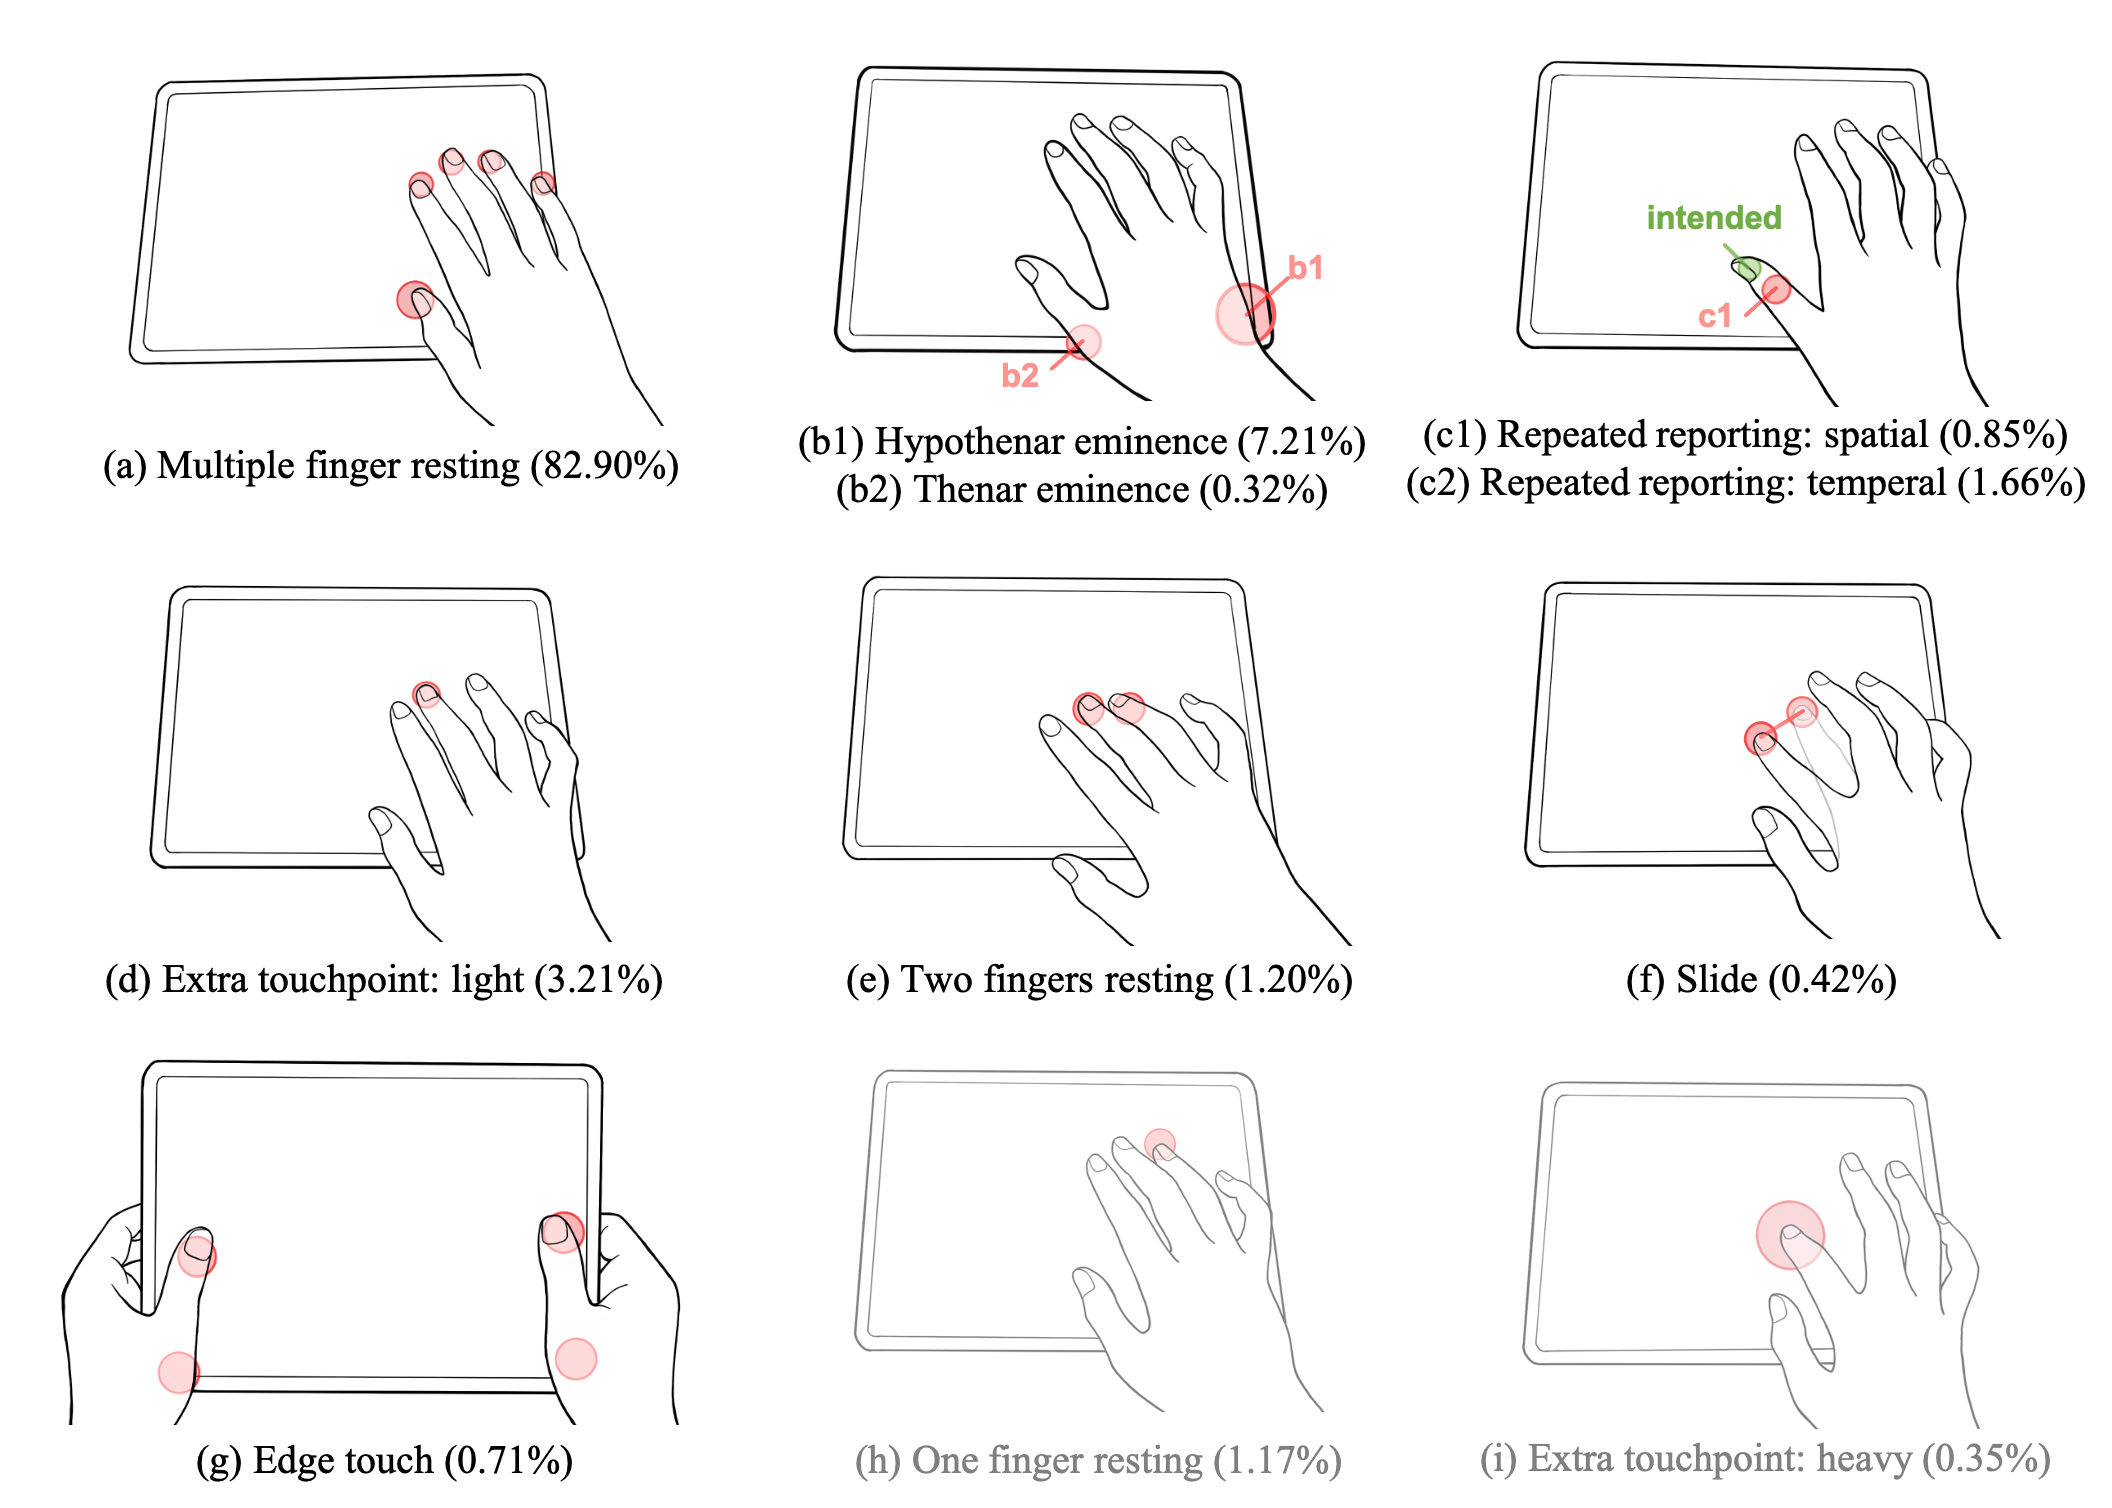
\includegraphics[width=1.0\linewidth]{figures/unintentional_touch.png}
	\centering
	\caption{各种可能的误触类型,和他们的频次,括号中的是该误触类型占总误触数量的比例。注意:1. 灰色(h,i)是理论不可分的;2. (d)Extra touchpoint和(h)单指resting的区别。3. c2没有被图示出来,具体是xxx的意思。4. 虽然双指/多指休息中,两个手指不可能是同时点上去的,但手指依次点下去的时间间隔大概率在100ms以内。}
	\label{fig:unintentional_touch}
\end{figure}

【图:三种硬件设置下算法的识别准确率,再用圆饼图画出误触和未识别的比例】

Figure xx shows that performances of our method among the three hardware settings. ANOVA shows a significant effect of hardware on the recognition accuracy (F, p). Bonferroni-corrected post-hoc tests showed significant differences between all hardware pairs: 1-2 (p<), 1-3 (p<), 2-3 (p<). Results show that the touchscreen devices with total pressure signal reach a balance between recognition accuracy and hardware cost.

Error rate (SD) / False Positive (SD) / False Negative (SD)
(1) 0.02028 0.01537 0.01262 0.01212 0.00766 0.00619
(2) 0.01392 0.01158 0.00876 0.01016 0.00516 0.00542
%(3) 0.01269 0.01175	0.0087 0.01055 0.00399 0.00396
(4) 0.01115 0.00726 0.00659 0.00578 0.00456 0.00451
